%TODO investigate the code repositories
%TODO define the common pattern for the server interaction
%TODO define request/response types(what can be combined, what cannot) for client part
%TODO update the report, add information about types to the server achitecture, introduce new problem if exists 
%TODO Make dependencies to the json tree*
%TODO update report with the algorithm of request aggregation 
%TODO integrate json tree* to the VIA app
%TODO update the report, add information about integration
%TODO set the web cache with for the dynamic and static content between via and clients
%TODO set the web cache between via and ovp
\section{Theory}
	
\subsection{Content Delivery Networks}


Nowadays the Internet is available from almost any place in the world. It allows people from different countries to communicate with each other and exchange information. The content providers and applications should serve the user's requests from all around the world with equally high speed in order to provide good user experience. In order to solve this task, companies should deploy their servers all around the world in multiple data centers. For world-class companies like Google and Netflix this task is solvable\cite{NetflixCDN}, but for middle-sized companies there should be another solution because it is very expensive and sometimes complicated to deploy servers in multiple data centers. Fortunately, the content delivery networks solve this problem\cite{AkamaiCDN}.

The Content Delivery Network(CDN) is a distributed system consisted of many servers deployed all around the world in different data centers. They act as a local content holders. The routes to the content providers and applications are configured to lay through the CDN's servers. When the client wants to access the server through the Internet, the request will be processed by the local CDN server; if it will find the data locally, it will deliver the response to the client without making the request to the content provider that can be located in different country. The CDNs can store both static and dynamic content. One of the first global solutions was presented by Akamai company\cite{AkamaiCDN}. The graphical architecture is depicted on figure \ref{fig:cdn_overview}.

The CDN consists of several parts: routing, load balancing, and web caching\cite{CDNOverview}. The web caching part will be reviewed because it is relevant to the project.

\begin{figure}[h]
    \centering
    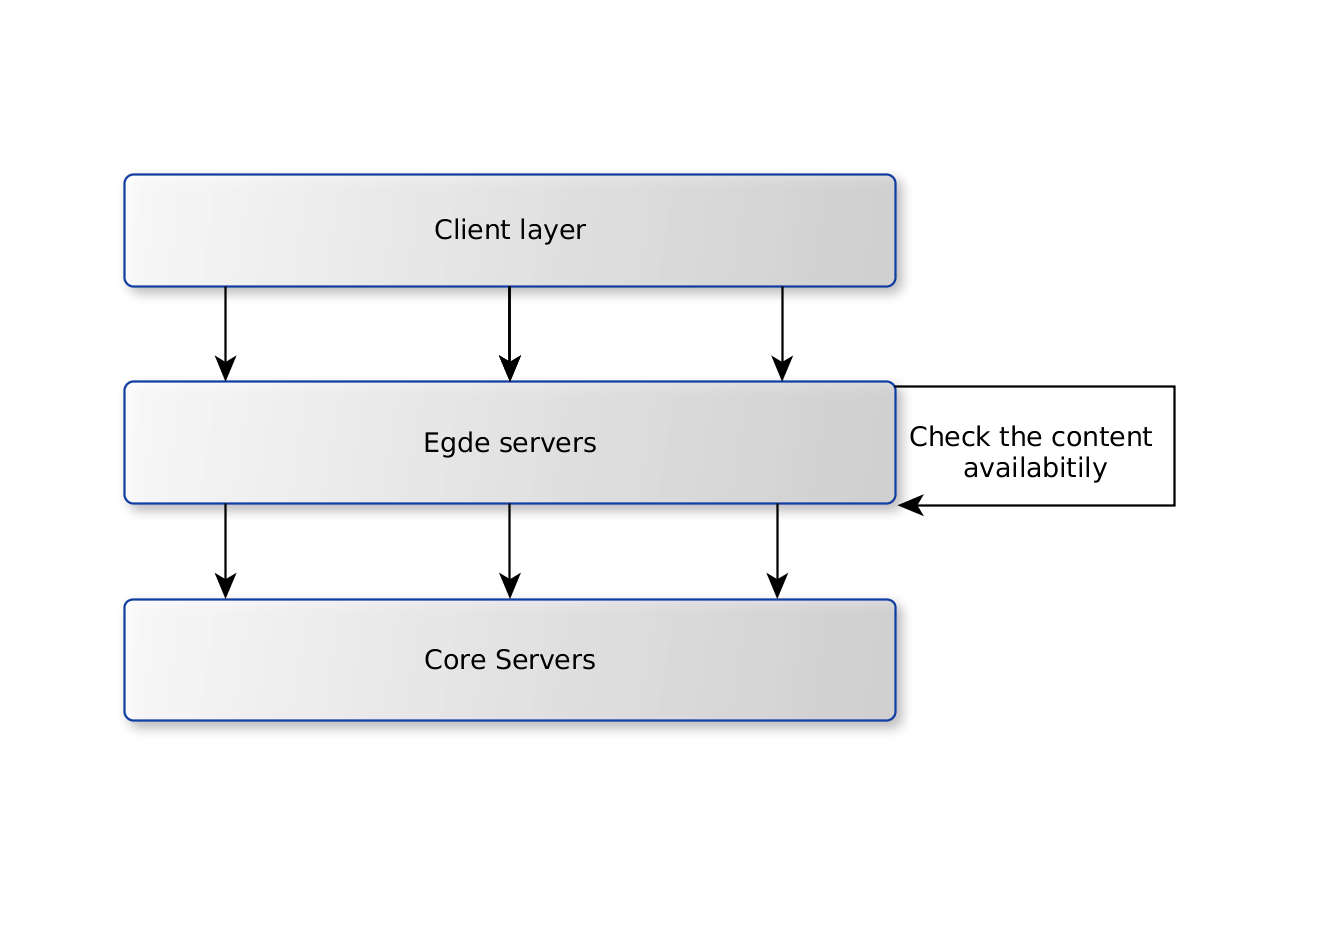
\includegraphics[width=\textwidth]{images/cdn_arch.png}
    \caption{Content Delivery Network Overview}
    \label{fig:cdn_overview}
\end{figure}

\subsection{Web Caching}

Web caching is the technique that allows to store temporary content that is requested from the Internet (e.g. HTML pages, JSON, XML or CSS files). It alleviates the server's work by reducing the amount of requests to it and reduces bandwidth usage\cite{WebCachingInterior}. A web cache system serves as a communication point between client and sevrer. The client's requests and server's responses are routed through it. The web cache stores responses from the server and returns them without hitting the underlying server. It also can manipulate the request/response headers.

The benefits of web caching:

\begin{itemize}
    \item Reduces the server workload; Using web caching the requests will go through the cache and will touch server only if the data does not present in caches or the data is stale. That will reduce the amount of requests made to server.
    \item Web caching improves user experience; The data will be delivered faster to the end users.
    \item Reduces bandwidth
\end{itemize}

\subsubsection{Content types}

% Describe static and dynamic content types

The content stored by web caches can be static or dynamic.

The static content is a set of resources that stay the same no matter what was the user input. Static objects are identified by the unique path and can be cached for a long time by the web caches.

The dynamic content is generated at run-time, based on the user input\cite{DynamicWebCaching}. The dynamic requests are almost always processed by servers. They are the main consumers of the web server's resources. The dynamic requests are time-dependent meaning that at different times the same request can produce different output; as a result, they cannot be cached for long periods of time by the web caches. Moreover, for security reasons, usually dynamic objects that contain client's personal data and preferences are configured in order to not be cached by the external web caches and CDNs.

However, almost all dynamic content is static for a short period of time. It changes only when the internal resources (e.g. databases) are altered. This gives a possibility to configure web cache for storing dynamic objects.

\subsubsection{Http Cache Control Headers}

Web cache is controlled by the http cache control headers\cite{RFC7234}. The control mechanisms can be specified on both request and response sides. There are several http headers that are relevant for the project: 
\begin{itemize}
    \item Cache-Control
    \item Vary header
    \item Etag, If-None-Match
    \item Last-Modified, If-Modified-Since
    \item Expires (for http 1.0)
    \item Widely used extension headers, like X-Cache.
\end{itemize}

There are two caching techniques: Time-based caching and Data-based caching.

The time-based caching is represented by the next http headers: \textit{Last-Modified} and \textit{If-Modified-Since}, \textit{Cache-Control} with \textit{s-maxage} parameter and \textit{Expires} header. The client sends the request with specified \textit{If-Modified-Since} header, where he indicates as a parameter the time when the content was modified. The server will then check the content type which was requested and send the corresponding response. If the static content was requested, the server will check if the resource was changed since the date specified by the client in \textit{If-Modified-Since} header, and will send the new content with the code 200 and updated \textit{Last-Modified} header if it was modified, otherwise it will reply with the code 304 (resource not modified) without content and with old \textit{Last-Modified} header. The server does not usually set the Last-Modified header to the dynamic resources because it is hard to know where exactly they were modified. 
During the response the server can specify the \textit{Cache-Control} header with s-maxage parameter. In this case, if the content is public, it can be cached by the web cache servers for s-maxage time specified in seconds. If the next request will occur in the next \textit{s-maxage} seconds, the content will be served from the web cache. This technique is used for caching both dynamic and static content. The difference between static and dynamic content is that the s-maxage parameter for the dynamic content is set dynamically, while it is set statically for the static content.

The data based caching is represented by the \textit{Etag} and \textit{If-None-Match} headers. It is supported since in HTTP/1.1. On the first request, the server will compute the hash of the content and send it to the client in the Etag header. The client will remember the hash value in the \textit{If-None-Match} header. When the next request occurs, the server will recompute the hash of the content and will compare it with the value specified in the \textit{If-None-Match} parameter. If the values are the same, the server will reply with the 304 code, without content and with the old Etag header; Otherwise it will change the Etag header to the new value and send the normal response. 


The web cache can be implemented on: 

\begin{itemize}
    \item Client side, by using browser caches
    \item Proxy servers, by introducing the middle caching server between client and server.
    \item Server side, by implementing cache programmatically
\end{itemize}

Currently, the middleware server supports the server side caching with Redis in memory data store. We will introduce the proxy server caching and will see if it will give the benefit to the architecture.(move to abstract) 

\subsubsection{An overview of proxy server types}

A proxy server is a server that is deployed between client and server. It acts as a middle point in communication between clients and servers. The proxy server redirects requests to servers and responses from servers to clients. It can improve the performance of the servers by storing the copies of frequently used resources. When a client makes a request to the server through the proxy server, the  proxy server serves as a web cache, it will try to find data locally and will return the resource back to the client with success.

There are two main types of proxy servers: forward and reversed proxy\cite{WWWCaching}.
A forward proxy is one of the most common types of proxy servers. The client is aware about the proxy server and can configure requests through it.
A reversed proxy is deployed by server administrators in the internal network. The client contacts the desired server, but the request is routed through the reversed proxy server. In this case, the client may not know about the underlying proxy. 
The reversed proxy server was selected for the project because it perfectly suits the architecture, the client should not know about the existence of the middle point. (and the web caching is mostly done by using reversed proxy servers).


\subsection{Http Session Management}

HTTP protocol is stateless by its nature, meaning that there is no possibility to distinguish one request from another. Http requests usually open new connection to the desired server every time. Nowadays, servers can specify \textit{Keep-Alive} header in the response in order to give browsers a hint that this connection can be used again for the new request. Unfortunately, without transferring user-specific information it is impossible to distinguish users.  

The session management is implemented through header fields  \textit{Set-Cookie} and \textit{Cookie} headers. When a server wants to distinguish one user from another it sets the unique identifiers for the user. This identifier is transferred in the header field Set-Cookie. The browser will parse this field and remember the unique identifier. For every new request, the browser will send this identifier its header field Cookie. Of course, the server can send additional information in Set-Cookie header that is unique for user. Unfortunately, it is very dangerous to transfer private information(e.g. credit card number) this way. The server can store a dictionary of user ids and corresponding private information in memory and retrieve this information every time when the browser specifies Cookie header. 


\newpage


